% 1. Nguyên, 2. Nhật, 3. Nhất, 4. Quân
\PassOptionsToPackage{table}{xcolor}
\documentclass{article}
\usepackage{style}
\usepackage{adjustbox}
\usepackage[utf8]{inputenc}
\usepackage[vietnamese]{babel}
\usepackage[T1]{fontenc}
\usepackage{hyperref}       % hyperlinks
\usepackage{url}            % simple URL typesetting
\usepackage{booktabs}       % professional-quality tables
\usepackage{amsfonts}       % blackboard math symbols
\usepackage{nicefrac}       % compact symbols for 1/2, etc.
\usepackage{microtype}      % microtypography
\usepackage{lipsum}		% Can be removed after putting your text content
\usepackage{float}
\usepackage{titlesec}
\usepackage{graphicx}
\usepackage{multicol}
\usepackage{eqparbox}
\usepackage{titletoc}
\usepackage{etoolbox}
\usepackage{tocloft}
\usepackage{enumerate}
\usepackage{doi}
\usepackage{xcolor}
\usepackage{float}
\usepackage{textpos}
\usepackage{algpseudocode}
\usepackage{algorithm}
\usepackage{import}
\usepackage{makeidx}
\usepackage[table]{xcolor}
\usepackage{eqparbox}
\usepackage[contents={}]{background}
\usepackage{amsmath,amsthm,amssymb}
\usepackage[shortlabels]{enumitem}
\usepackage{caption}
\usepackage{setspace}
\usepackage{tocloft}
\usepackage{minted}
\usepackage{tkz-tab}
\usepackage{tikz,pgf}
\usepackage{fancyhdr}
\usepackage{tikz}
\usepackage{multirow}

\usepackage[style=ieee]{biblatex}
\addbibresource{references.bib}

% Adjust the spacing before and after section and subsection titles
\titlespacing*{\section}{0pt}{*0.5}{*0.5}
\titlespacing*{\subsection}{0pt}{*0.5}{*0.5}
\usetikzlibrary{shapes.geometric, arrows.meta, positioning}
\let\oldbib\thebibliography

\renewcommand*{\bibfont}{\Large} % Change \normalsize to the desired font size

\tikzstyle{startstop} = [rectangle, rounded corners, minimum width=4cm, minimum height=1.5cm, text centered, text width=7cm, draw=black, fill=green!30]
\tikzstyle{process} = [rectangle, rounded corners, minimum width=4cm, minimum height=1.5cm, text centered, text width=5cm, draw=black, fill=green!30]
\tikzstyle{arrow} = [thick,->,>=stealth]


\makeindex
\rhead{CS336.P11 - UIT}

%\captionsetup[table]{position=bottom}
\numberwithin{equation}{section}
\titlecontents{section}[0em]
{\vskip 0.5ex}%
{\scshape}% numbered sections formatting
{\itshape}% italics sections formatting
{}%
% \fancyhf{}
% \rhead{\footnotesize\nouppercase\rightmark} % Bên phải header: tên section
% \lhead{\footnotesize\nouppercase\leftmark} % Bên trái header: tên chapter
% \cfoot{\footnotesize\thepage} % Giữa footer: số trang

% Tùy chỉnh định dạng của các phần trong mục lục
\renewcommand{\cftsecfont}{\Large\bfseries}
\renewcommand{\cftsubsecfont}{\large\bfseries}
\renewcommand{\cftsubsubsecfont}{\normalsize\bfseries}

\renewcommand{\cftsecpagefont}{\Large\bfseries}
\renewcommand{\cftsubsecpagefont}{\large\bfseries}
\renewcommand{\cftsubsubsecpagefont}{\normalsize\bfseries}

\renewcommand{\cftsecafterpnum}{\cftdotfill{\cftdotsep}}
\renewcommand{\cftsubsecafterpnum}{\cftdotfill{\cftdotsep}}
\renewcommand{\cftsubsubsecafterpnum}{\cftdotfill{\cftdotsep}}

\cftsetindents{section}{0em}{4em}
\cftsetindents{subsection}{2em}{4em}
\cftsetindents{subsubsection}{4em}{4em}

% Ensure section numbers have a dot after them
\renewcommand{\cftsecaftersnum}{.}
\renewcommand{\cftsubsecaftersnum}{.}
\renewcommand{\cftsubsubsecaftersnum}{.}
\renewcommand{\cftsecnumwidth}{2.3em}

\numberwithin{equation}{section}
\setcounter{secnumdepth}{4}
\setcounter{tocdepth}{4}
\renewcommand{\contentsname}{Mục lục}



\begin{document}
\begin{titlepage}
\import{./}{cover.tex}
\end{titlepage}
\clearpage
\newpage
\LARGE
\setcounter{page}{1}
\tableofcontents
\clearpage
\newpage
\Large
% ---- START HERE ------------------------------- 
\setstretch{1.2}
\section{\textbf{Giới thiệu}}
\subsection{Giới thiệu đề tài}
Trong bối cảnh hiện đại, với sự phát triển mạnh mẽ của trí tuệ nhân tạo (AI) đã mở ra những cơ hội mới để nâng cao trải nghiệm khách hàng trong các lĩnh vực kinh doanh. Một trong những ứng dụng nổi bật là chatbot – hệ thống tự động giao tiếp thông minh, có khả năng cung cấp thông tin và hỗ trợ khách hàng một cách nhanh chóng và hiệu quả.

Đề tài \textbf{“Xây dựng hệ thống Chatbot tư vấn khách hàng về sản phẩm thảo dược”} được thực hiện với mục tiêu phát triển một công cụ hỗ trợ giao tiếp giữa doanh nghiệp và khách hàng. Cửa hàng thảo dược, với đặc thù sản phẩm liên quan đến sức khỏe và yêu cầu tư vấn chính xác, là môi trường lý tưởng để áp dụng công nghệ này. Hệ thống chatbot không chỉ giúp giảm tải công việc cho nhân viên, mà còn đảm bảo khả năng cung cấp thông tin kịp thời và chính xác về công dụng, cách sử dụng và đặc điểm của các sản phẩm thảo dược.

Với bài toán này, nhóm sẽ ứng dụng mô hình \textbf{Retrieval-Augmented Generation (RAG)} – một phương pháp kết hợp giữa khả năng truy xuất thông tin (Information Retrieval) và sinh văn bản tự nhiên (Generation). Mô hình RAG cho phép chatbot truy vấn cơ sở dữ liệu nội bộ của cửa hàng để lấy thông tin chi tiết về các sản phẩm thảo dược, sau đó sử dụng khả năng sinh ngôn ngữ tự nhiên để trả lời khách hàng một cách mạch lạc và chính xác. Cách tiếp cận này không chỉ giúp chatbot giải đáp các câu hỏi thường gặp mà còn cung cấp các tư vấn mang tính cá nhân hóa, đáp ứng nhu cầu đa dạng của người tiêu dùng.

Thông qua việc áp dụng công nghệ RAG, hệ thống chatbot được kỳ vọng sẽ mang lại sự đột phá trong việc cải thiện chất lượng phục vụ khách hàng. Không chỉ hỗ trợ quá trình mua sắm, chatbot còn giúp nâng cao nhận thức của khách hàng về các sản phẩm thảo dược và lợi ích của việc sử dụng chúng trong chăm sóc sức khỏe.

\subsection{Lý do chọn đề tài}
Đề tài này được lựa chọn với mong muốn giải quyết các vấn đề thông qua việc áp dụng công nghệ hiện đại. Việc phát triển hệ thống chatbot mang lại nhiều lợi ích thiết thực:
\begin{itemize}
    \item \textbf{Tăng trải nghiệm khách hàng:} Hệ thống chatbot sẽ cung cấp thông tin chính xác, tư vấn cá nhân hóa dựa trên nhu cầu của từng khách hàng, từ đó nâng cao sự hài lòng của khách hàng đối với sản phẩm và dịch vụ của cửa hàng.
    \item \textbf{Hỗ trợ khách hàng 24/7:} Chatbot hoạt động liên tục, không bị giới hạn bởi thời gian hay không gian, đảm bảo khách hàng có thể nhận được sự hỗ trợ bất cứ lúc nào. Điều này đặc biệt hữu ích trong bối cảnh kinh doanh trực tuyến ngày càng phổ biến.
    \item \textbf{Giảm tải công việc cho nhân viên tư vấn:} Với khả năng xử lý khối lượng lớn các câu hỏi lặp lại, chatbot giúp nhân viên tập trung vào các nhiệm vụ phức tạp và mang tính chuyên sâu hơn, từ đó cải thiện hiệu suất làm việc.
\end{itemize}
Với các lý do trên, đề tài này không chỉ có giá trị thực tiễn cao mà còn góp phần thúc đẩy sự phát triển của AI trong lĩnh vực kinh doanh thảo dược, mang lại lợi ích thiết thực cho cả doanh nghiệp và khách hàng.

\subsection{Giới thiệu bộ dữ liệu}
Bộ dữ liệu được sử dụng trong nghiên cứu này bao gồm thông tin chi tiết của 105 sản phẩm từ website cửa hàng Toàn Thắng: \texttt{\url{https://tratoanthang.com/}}, một đơn vị chuyên kinh doanh các mặt hàng thảo dược. Bộ dữ liệu tập trung vào các sản phẩm thuộc danh mục: trà thảo dược, cao atisô, và các sản phẩm thảo dược khác.

Mỗi mục dữ liệu trong bộ này cung cấp thông tin đầy đủ và chi tiết về từng sản phẩm, bao gồm:

\begin{itemize}
    \item \textbf{Tên sản phẩm:} Định danh sản phẩm cụ thể.
    \item \textbf{Tình trạng:} Thông tin về tình trạng sẵn có của sản phẩm (còn hàng hoặc hết hàng).
    \item \textbf{Giá:} Giá gốc của sản phẩm.
    \item \textbf{Giá khuyến mãi (nếu có):} Giá giảm trong các chương trình ưu đãi.
    \item \textbf{Mô tả thành phần:} Thông tin về các thành phần chính tạo nên sản phẩm.
    \item \textbf{Công dụng:} Các lợi ích và hiệu quả của sản phẩm đối với sức khỏe người dùng.
\end{itemize}

Hình~\ref{fig:product-example} thể hiện thông tin chi tiết về một sản phẩm trong bộ dữ liệu.

\begin{figure}[!ht]
    \centering
    \adjustbox{max width=1\linewidth, keepaspectratio}{%
        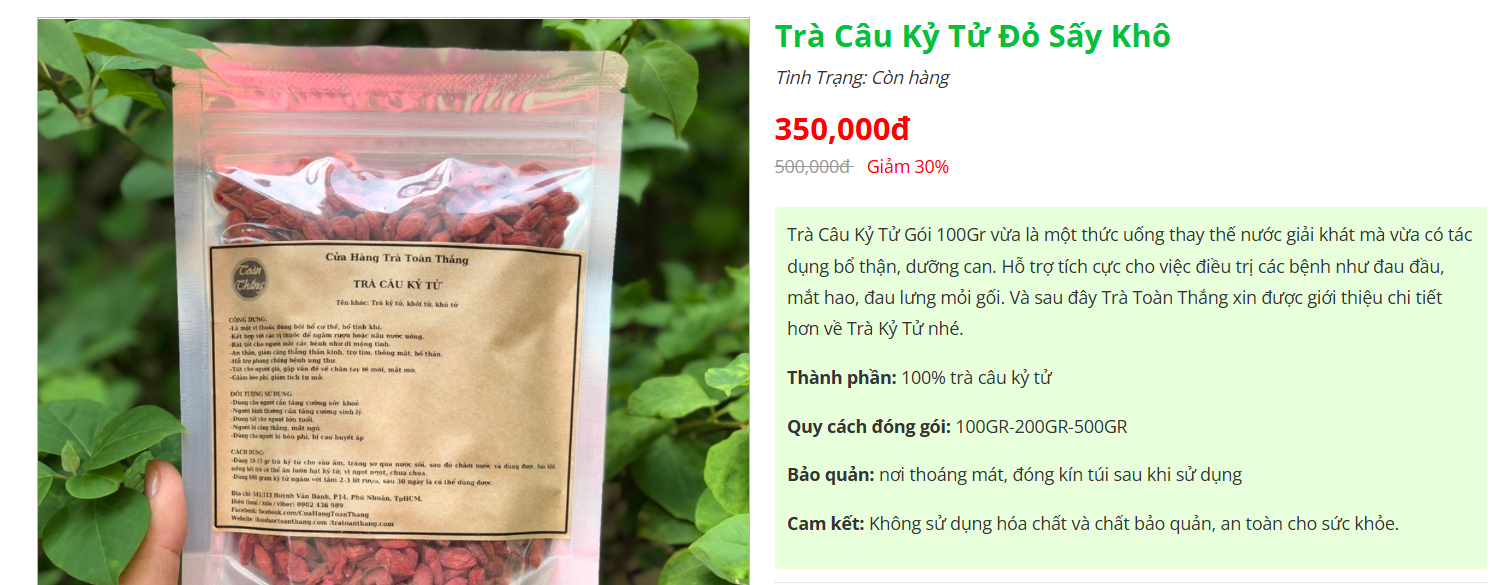
\includegraphics{images/product-example.png}%
    }
    \caption{Hình ảnh về thông tin của một sản phẩm}
    \label{fig:product-example}
\end{figure}

\section{\textbf{Quy trình}}
Quy trình xây dựng Chatbot được nhóm thực hiện qua hai quy trình: Quy trình thu thập và xử lý dữ liệu~\ref{fig:data-pipeline}, Quy trình Chatbot hoạt động~\ref{fig:chatbot-pipeline}.
\begin{figure}[!ht]
    \centering
    \adjustbox{max width=1\linewidth, keepaspectratio}{%
        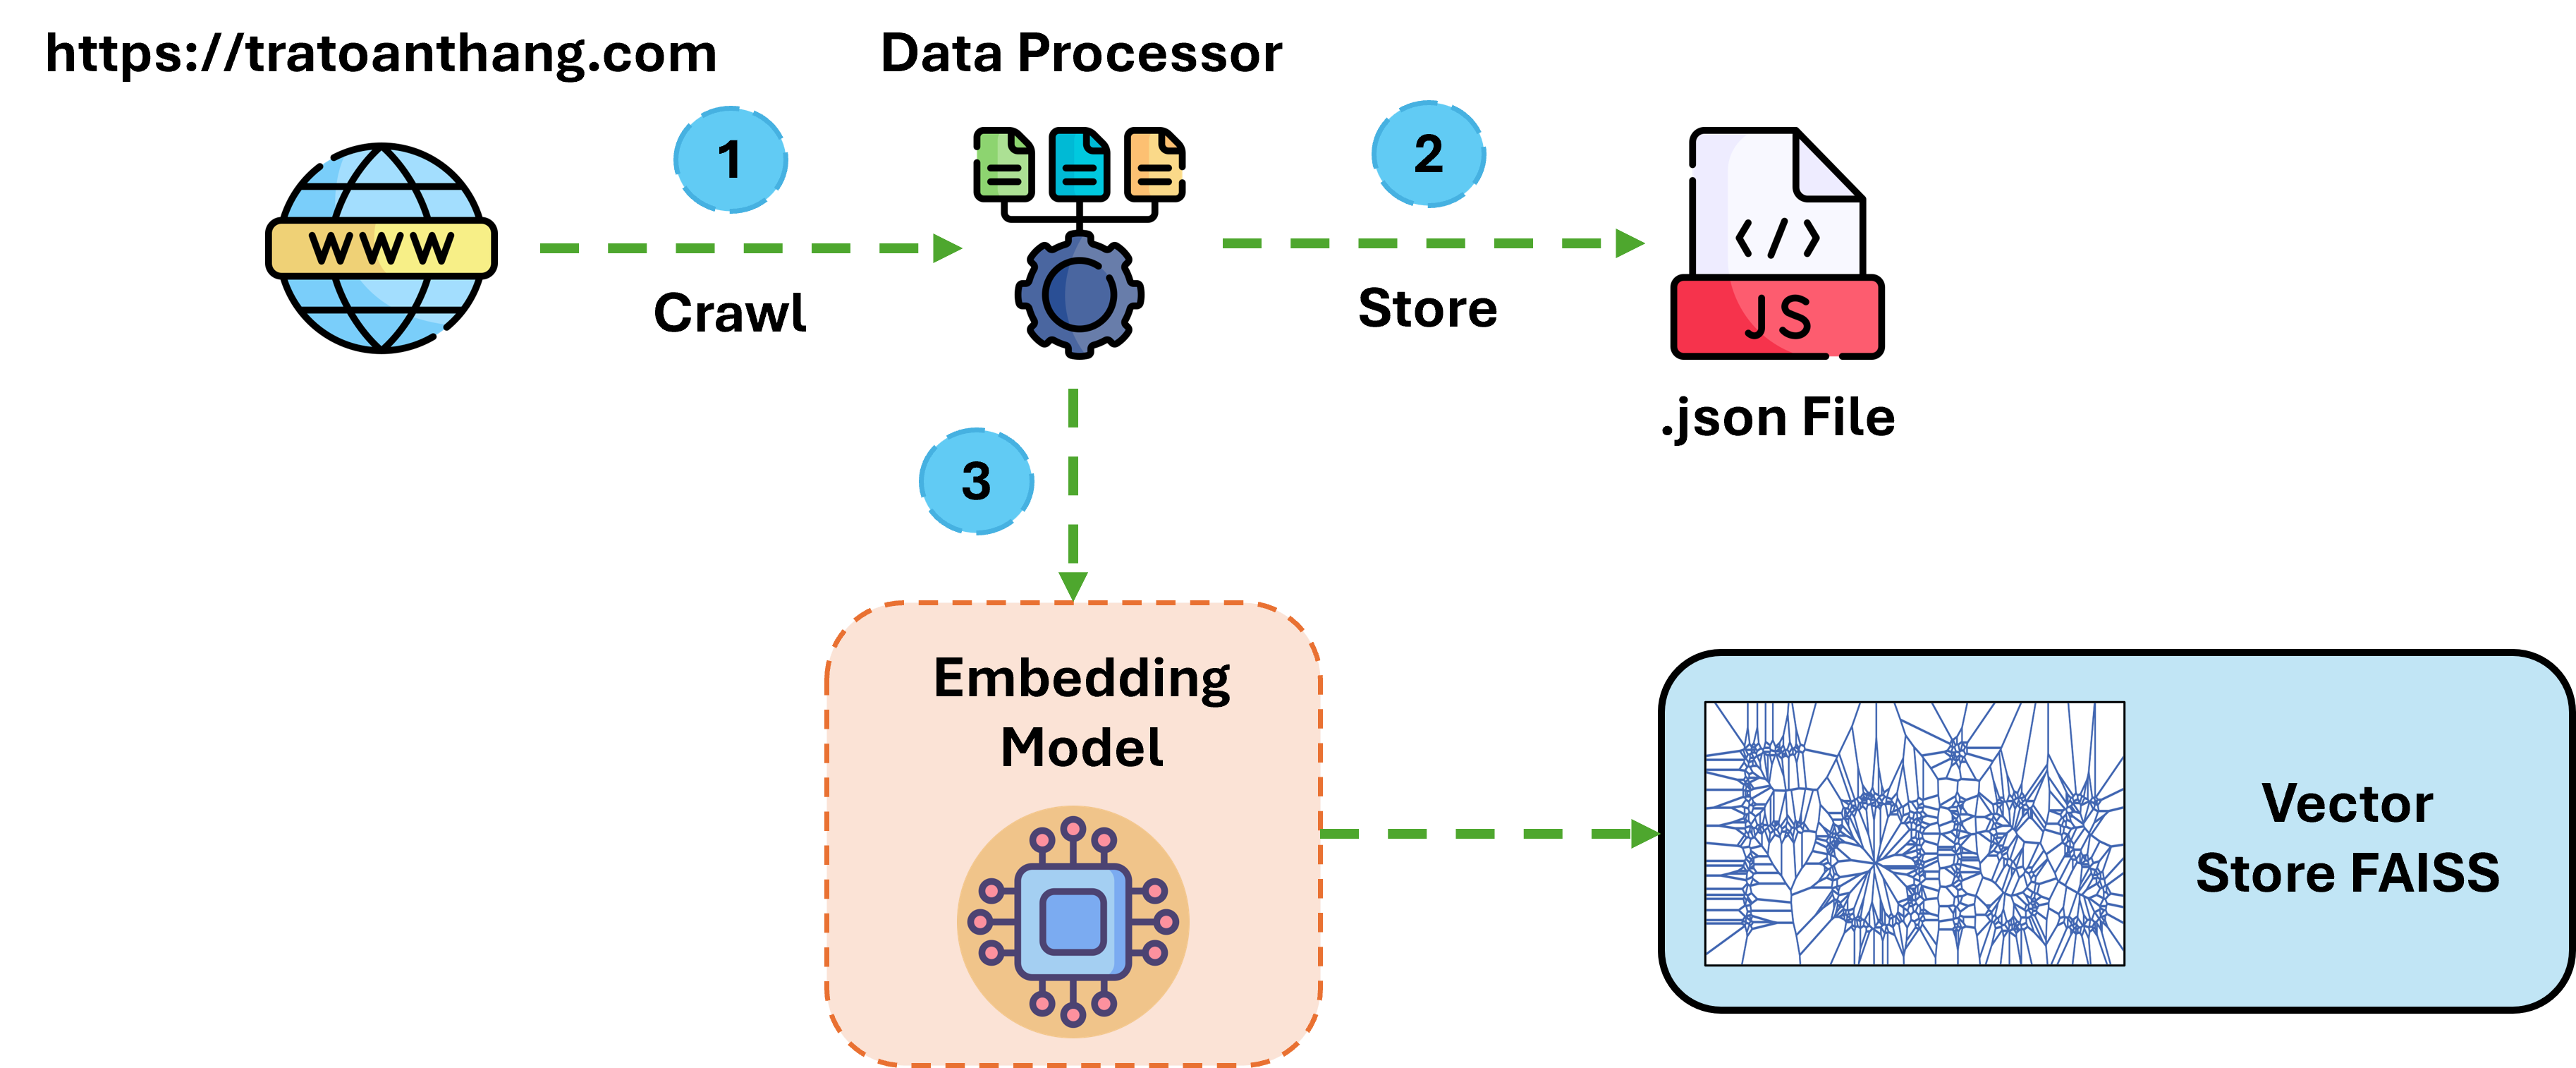
\includegraphics{images/data_pipeline.png}%
    }
    \caption{Quy trình thu thập và xử lý dữ liệu}
    \label{fig:data-pipeline}
\end{figure}
\subsection{Thu thập dữ liệu}

Với mong muốn có được những dữ liệu thực tế và sát với yêu cầu của hệ thống Chatbot tư vấn về các sản phẩm thảo dược, nhóm đã tìm hiểu và khảo sát rất nhiều website bán hàng có sản phẩm liên quan. Website mà nhóm chọn để lấy dữ liệu và tiến hành xây dựng Chatbot để truy vấn là website: \texttt{\url{https://tratoanthang.com/}} vì độ đa dạng sản phẩm cũng như độ uy tín cao của cửa hàng. Một số sản phẩm của cửa hàng được ví dụ ở hình ~\ref{fig:website-products}.

\begin{figure}[!ht]
    \centering
    \adjustbox{max width=1\linewidth, keepaspectratio}{%
        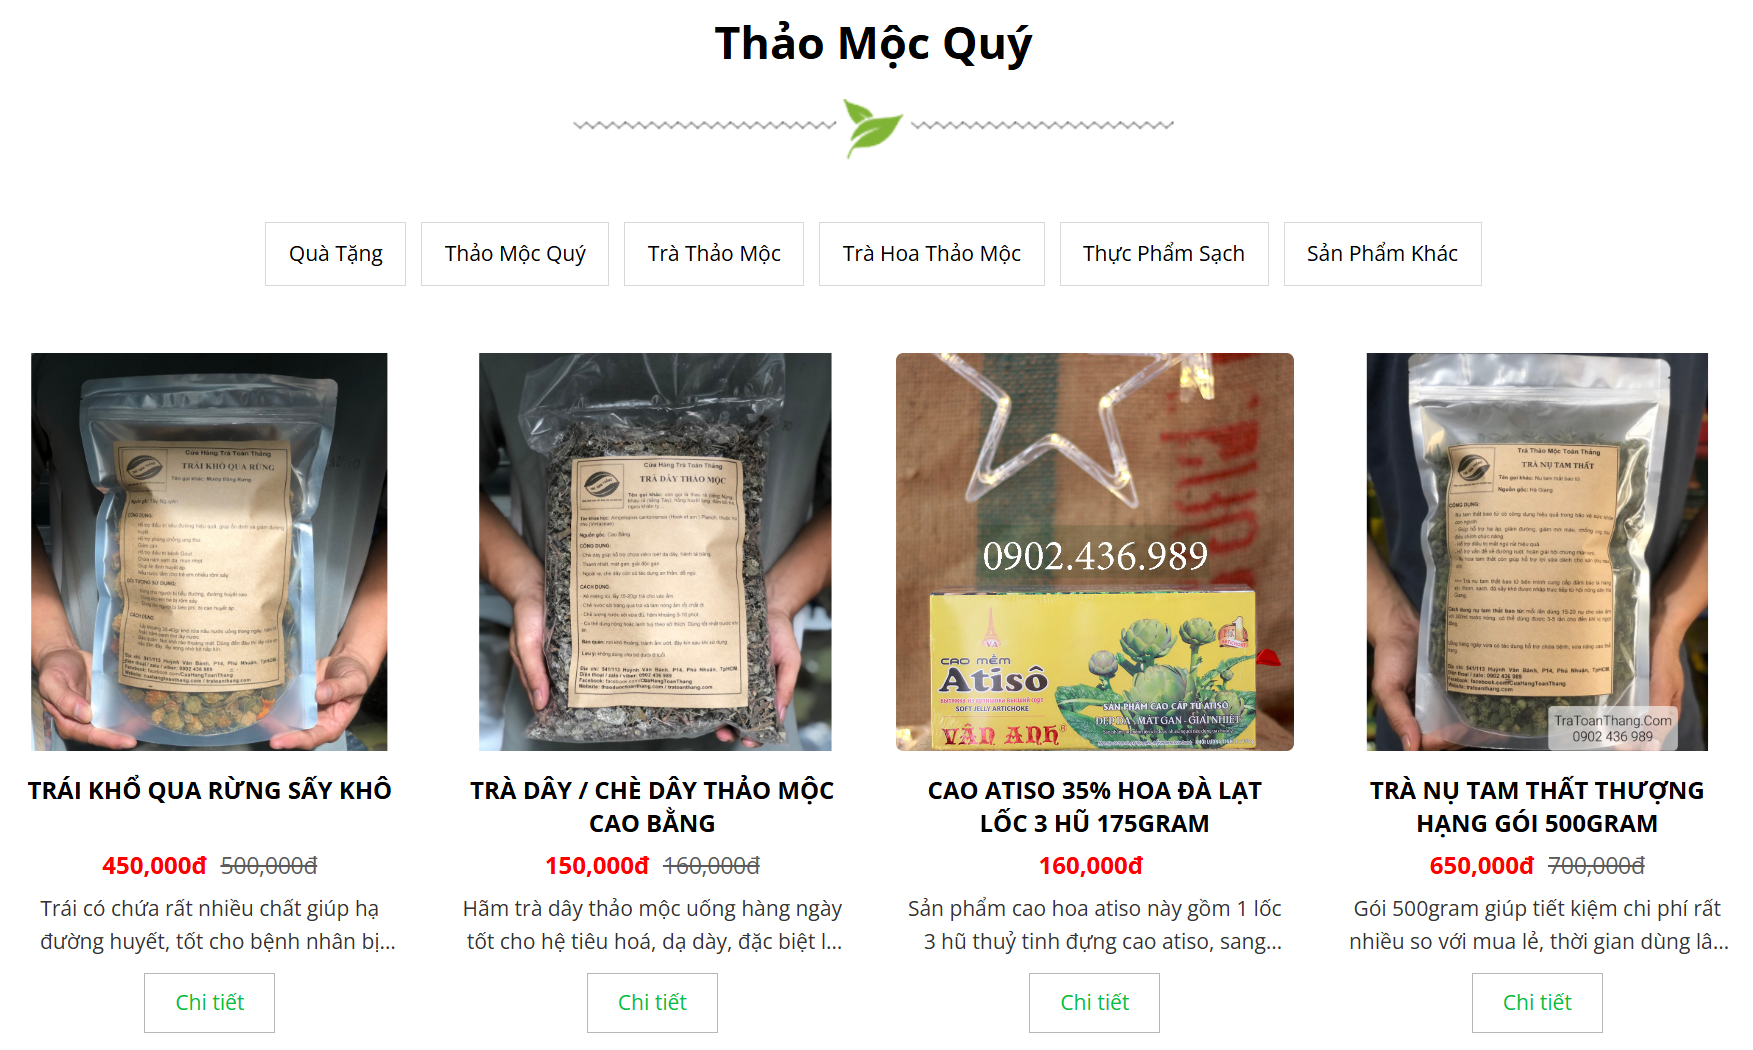
\includegraphics{images/website-products.png}%
    }
    \caption{Hình ảnh một số sản phẩm từ website \texttt{\url{https://tratoanthang.com/}}}
    \label{fig:website-products}
\end{figure}

Sau khi chọn được nguồn dữ liệu phù hợp với đề tài, nhóm tiến hành xây dựng một crawler để thu thập dữ liệu từ website. Crawler được xây dựng bằng các thư viện Selenium cùng BeautifulSoup. 

Để dữ liệu thu thập được thật sự hiệu quả và nhất quán, nhóm tiến hành loại bỏ các tags \texttt{HTML} và Chuẩn hóa các giá trị liên quan đến giá cả, văn bản tiếng Việt như một bước tiền xử lý trước khi dữ liệu được lưu lại dưới dạng \texttt{json}. Hình~\ref{fig:data-example} thể hiện một mẩu dữ liệu mà nhóm đã thu thập được sau khi trải qua bước tiền xử lý.

\begin{figure}[!ht]
    \centering
    \adjustbox{max width=1\linewidth, keepaspectratio}{%
        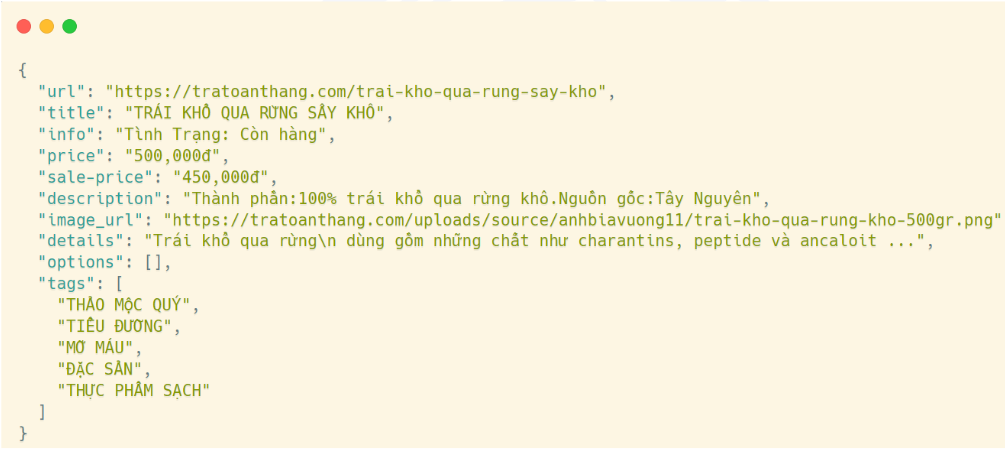
\includegraphics{images/data-example.png}%
    }
    \caption{Hình ảnh ví dụ về một mẩu dữ liệu}
    \label{fig:data-example}
\end{figure}
\subsection{Xử lý dữ liệu}
Nhóm sử dụng các trường dữ liệu: \textbf{Tên sản phẩm, Giá gốc, giá khuyến mãi, Danh mục sản phẩm, Mô tả} và \textbf{Thông tin chi tiết} để truy xuất. Trong đó \textbf{Tên sản phẩm, Giá gốc, giá khuyến mãi, Mô tả} và \textbf{Thông tin chi tiết} là những thông tin đã có sẵn sau bước thu thập dữ liệu, còn Danh mục sản phẩm là một trường dữ liệu mới do nhóm tiến hành xử lý dữ liệu mà phân ra dựa trên loại sản phẩm. Danh mục sản phẩm bao gồm: 
\begin{itemize}[-]
    \item \textbf{"Sản phẩm Trà"}: Các sản phẩm có dạng trà/túi lọc trà, ví dụ: "Trà xanh gạo rang - GENMAICHA", "Trà túi lọc cung đình Huế", ...
    \item \textbf{"Sản phẩm dạng Bột"}: Các sản phẩm có dạng bột, ví dụ: "Bột sắn dây nguyên chất", "Bột tam thất bắc hũ 200 gram", ...
    \item \textbf{"Sản phẩm dạng Cao"}: Các sản phẩm có dạng cao, ví dụ: "Cao Atiso 95\% lá Đà Lạt (hộp đen)",  "Cao Atiso 35\% hoa hộp 500 gram", ...
    \item \textbf{"Sản phẩm dạng Viên"}: Các sản phẩm có dạng viên, ví dụ: "Viên Trinh Nữ Hoàng Cung Cao Xạ Đen", "Viên Hà Thủ Ô Mật Ong Rừng - Giúp Đen Tóc Đỏ Da", ...
    \item \textbf{"Sản phẩm Combo"}: Các sản phẩm đi theo combo, ví dụ: "Combo 12 loại trà hoa set sẵn - An Hoa".
    \item \textbf{"Sản phẩm khác"}: Các sản phẩm khác không thuộc những danh mục trên, ví dụ: "Lá xạ đen khô Hòa Bình", "Hà thủ ô chế đậu đen"
\end{itemize}

Với những trường dữ liệu đã trình bày phía trên, nhóm cho rằng Chatbot có thể cung cấp cho khách hàng những thông tin cần thiết về sản phẩm của cửa hàng khi được truy vấn. 

Sau khi đã xác định được các trường dữ liệu cần thiết, nhóm áp dụng kỹ thuật Chunking để chia dữ liệu thành các chunks nhỏ hơn. Kỹ thuật này sẽ được trình bày rõ hơn ở phần \textbf{Phương pháp và Kỹ thuật}. Nhóm chọn phương pháp chunking một trong những phương pháp chunking hiệu quả nhất hiện tại là Semantic Chunking. Các chunks dữ liệu này sẽ được mã hóa bằng các embedding thành các vector embedding sau đó được lưu vào vector store FAISS~\cite{douze2024faisslibrary}.
\subsection{Quy trình hoạt động}

Chatbot mà nhóm đã xây dựng được hoạt động theo một quy trình cơ bản và dễ hiểu như ở hình~\ref{fig:chatbot-pipeline}. Các bước cụ thể như sau:
\begin{figure}[!ht]
    \centering
    \adjustbox{max width=1\linewidth, keepaspectratio}{%
        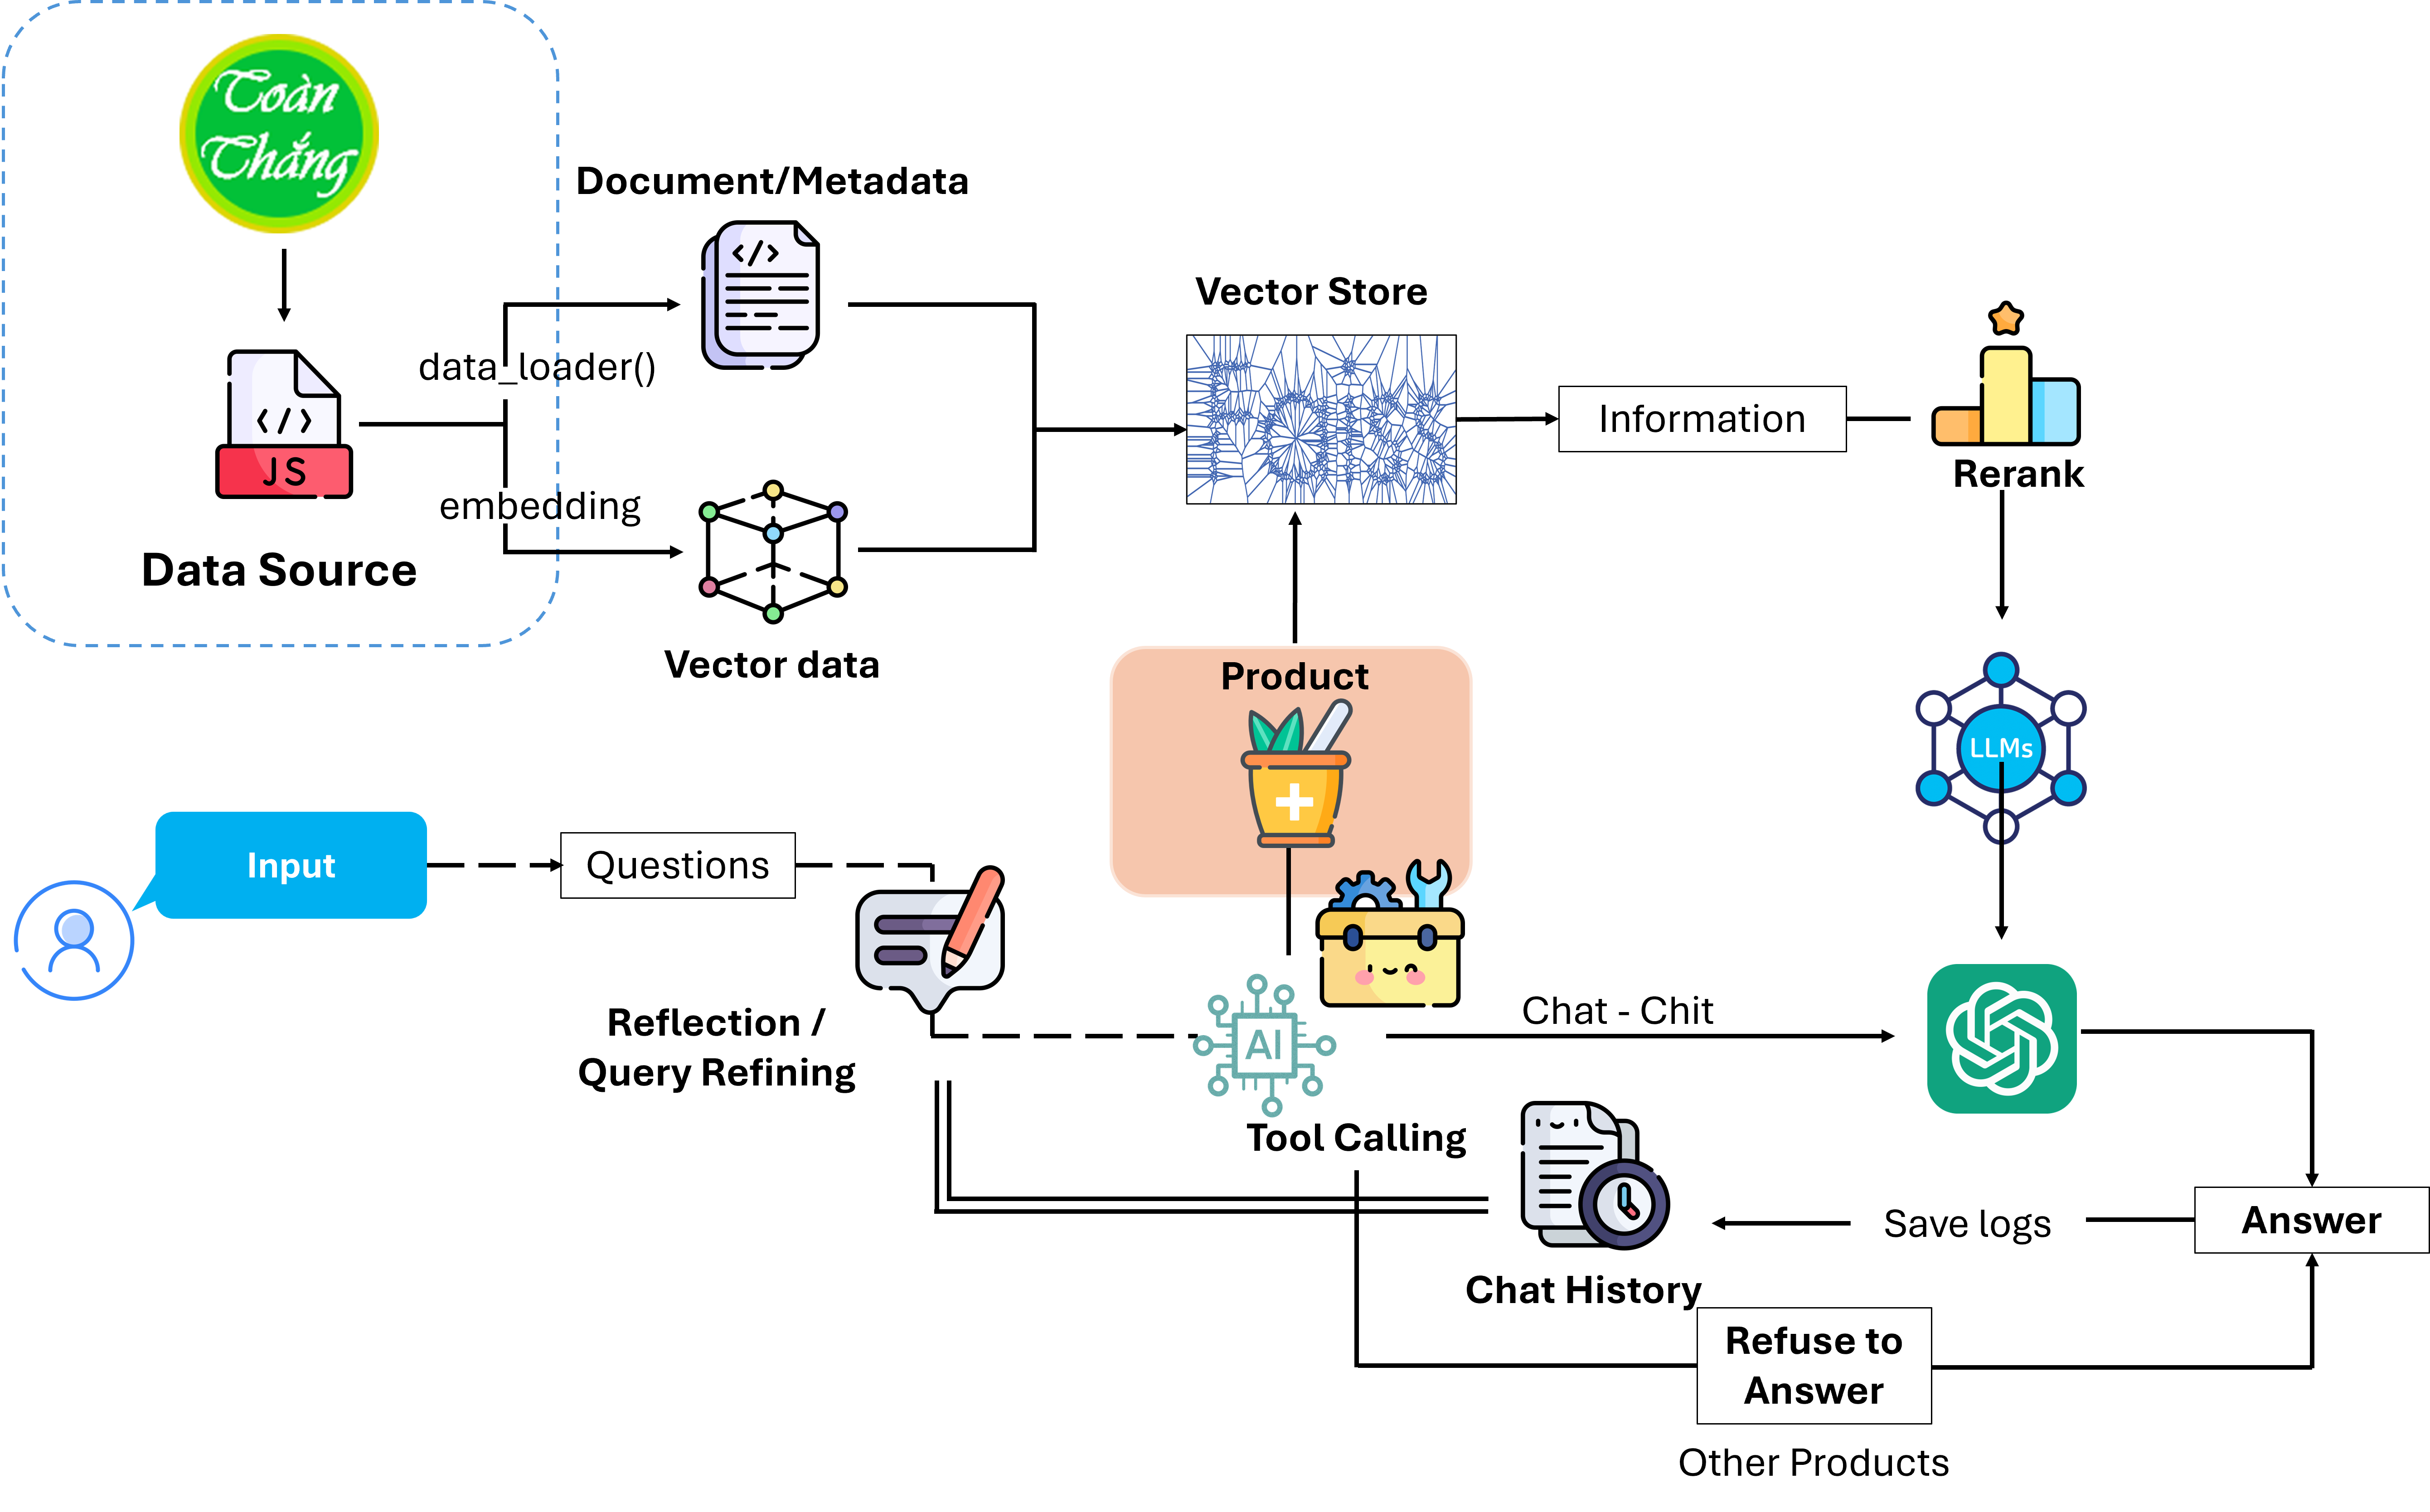
\includegraphics{images/chatbot_pipeline.png}%
    }
    \caption{Quy trình Chatbot hoạt động}
    \label{fig:chatbot-pipeline}
\end{figure}
\begin{enumerate}
    \item Người dùng đặt các câu hỏi cho Chatbot. Sau khi nhận được câu hỏi của người dùng, Chatbot sẽ sử dụng kỹ thuật \textbf{Reflection} (sẽ trình bày rõ hơn ở phần \textbf{Phương pháp và kỹ thuật}) để tổng hợp lại câu hỏi cùng với lịch sử trò chuyện của người dùng trước đó để chỉnh sửa câu truy vấn/prompt cho thật sự phù hợp với ngữ cảnh. 
    \item Câu prompt (đã được điều chỉnh) sẽ được đưa qua một mô hình ngôn ngữ lớn để xác định câu prompt đó thuộc nhóm nào trong số: "Câu hỏi về sản phẩm thảo dược \textbf{(1)}", "Câu hỏi về một loại sản phẩm khác \textbf{(2)}", "Câu hỏi xã giao/không liên quan đến sản phẩm \textbf{(3)}". Dựa vào đó mà Chatbot sẽ sử dụng đến một trong các "Tool" đã được định nghĩa sẵn và đi đến các trường hợp như sau:
    \begin{enumerate}[(1)]
        \item Tìm kiếm các sản phẩm có liên quan đến câu truy vấn trong vector store đã được lưu trữ bằng các phương pháp tìm kiếm. Sau khi lấy được thông tin cần thiết, sử dụng kỹ thuật \textbf{Reranking} bằng một \textbf{Reranker} (sẽ được trình bày rõ hơn ở phần \textbf{Phương pháp và Kỹ thuật} để tăng cường tính đúng đắn và mức độ liên quan, tối ưu hóa kết quả thông tin được truy vấn. Cuối cùng, một mô hình ngôn ngữ lớn khác sẽ được sử dụng để tạo ra câu trả lời liên quan cho khách hàng dựa trên thông tin đã được truy vấn. Ngoài ra, nếu câu truy vấn có liên quan đến việc khách hàng mong muốn mua sản phẩm từ cửa hàng, Chatbot sẽ tiến hành cung cấp thông tin về SĐT và Email cửa hàng cho khách hàng.
        \item Chatbot từ chối trả lời câu hỏi một cách lịch sử và khéo léo dẫn dắt người dùng quay về cuộc hội thoại về sản phẩm thảo dược.
        \item Chatbot vẫn sẽ sẵn sàng trả lời một vài câu hỏi xã giao bằng một mô hình ngôn ngữ lớn như trên, tuy nhiên sau đó sẽ khéo léo dẫn dắt người dùng quay về cuộc hội thoại về sản phẩm thảo dược.
    \end{enumerate}
    \item Cuối cùng, câu prompt và câu trả lời được Chatbot trả ra sẽ được lưu lại vào lịch sử trò chuyện của khách hàng.
\end{enumerate}
\section{\textbf{Phương pháp và Kỹ thuật}}
Dưới đây là một số kỹ thuật và phương pháp nhóm đã sử dụng trong đề tài này.

\subsection{Reflection}
\textbf{Reflection}~\ref{fig:reflection} là quá trình mà thay vì chỉ đơn thuần sử dụng câu hỏi gốc, Chatbot cần phải "suy nghĩ" về câu hỏi đó, kết hợp với lịch sử hội thoại, để tạo ra một truy vấn tinh chỉnh và phù hợp hơn với ngữ cảnh và mục tiêu của người dùng. Sau đó sử dụng prompt này đưa vào hệ thống RAG để tạo ra câu trả lời có độ chính xác hơn và phù hợp với ngữ cảnh.

\begin{figure}[!ht]
    \centering
    \adjustbox{max width=1\linewidth, keepaspectratio}{%
        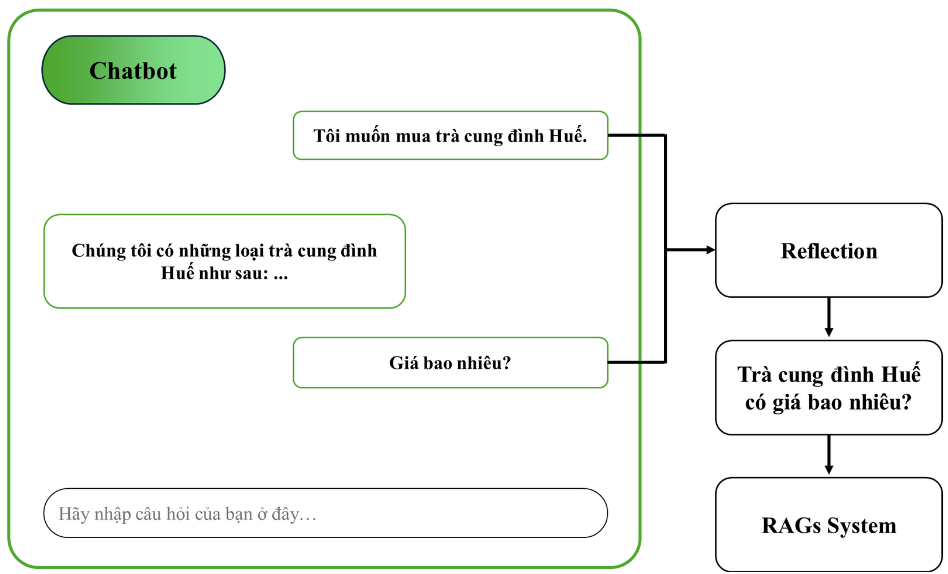
\includegraphics{images/reflection.png}%
    }
    \caption{Ví dụ cách Reflection hoạt động}
    \label{fig:reflection}
\end{figure}

Khi người dùng đưa ra một câu hỏi, Chatbot không trực tiếp sử dụng câu hỏi đó để tìm kiếm thông tin. Thay vào đó, chatbot sẽ thực hiện các bước sau:

\begin{enumerate}
\item \textbf{Phân tích câu hỏi gốc:} Hiểu ý định và mục đích chính của người dùng thông qua câu hỏi.
\item \textbf{Xem lại lịch sử hội thoại:} Tham khảo các câu hỏi và câu trả lời trước đó trong phiên trò chuyện để nắm bắt ngữ cảnh hội thoại và duy trì mạch lạc.
\item \textbf{Tổng hợp và tinh chỉnh truy vấn:} Kết hợp thông tin từ câu hỏi gốc và lịch sử hội thoại để tạo ra một truy vấn mới, rõ ràng và phù hợp ngữ cảnh trò chuyện hơn.
\end{enumerate}

Ví dụ, nếu người dùng hỏi: \textit{"Tôi muốn tìm trà thảo dược cho người mất ngủ"} và trước đó đã hỏi về \textit{"các loại trà tốt cho sức khỏe"}. Kỹ thuật Reflection có thể giúp chatbot nhận ra rằng người dùng đang muốn tìm kiếm \textbf{cụ thể} trà thảo dược và \textbf{đặc biệt} là loại trà giúp cải thiện giấc ngủ. Dựa trên đó, chatbot có thể tạo ra một truy vấn tinh chỉnh hơn như: \textit{"Trà thảo dược hỗ trợ giấc ngủ"} hoặc \textit{"Các loại trà thảo dược tốt cho người mất ngủ"}.

\subsection{Chunking: Semantic Chunking}
Do Chatbot được xây dựng trên mô hình RAG, \textbf{Chunking}~\cite{Saxena2023ChunkingRAG}~\cite{Bouchard2023RAGChunking} là một bước quan trọng trong quá trình xử lý dữ liệu trước khi đưa vào vector store. Chunking là quá trình phân chia dữ liệu văn bản lớn thành các đoạn nhỏ hơn, gọi là \textbf{chunks} (đoạn). Mục tiêu của chunking là tối ưu hóa hiệu quả của quá trình truy xuất thông tin và sinh văn bản.

Việc chia nhỏ văn bản mang lại nhiều lợi ích:
\begin{itemize}[-]
    \item \textbf{Tăng độ chính xác truy xuất:} Các chunk nhỏ hơn, tập trung vào một đoạn thông tin cụ thể, giúp quá trình tìm kiếm trở nên chính xác hơn. Thay vì tìm kiếm trên toàn bộ văn bản dài, hệ thống RAG có thể tập trung vào các chunk nhỏ, tăng khả năng tìm thấy thông tin liên quan đến câu hỏi của người dùng.
    \item \textbf{Phù hợp với giới hạn ngữ cảnh của mô hình ngôn ngữ:} Các mô hình ngôn ngữ lớn (LLMs) thường có giới hạn về độ dài ngữ cảnh (context window). Việc chia văn bản thành các chunk nhỏ giúp đảm bảo rằng thông tin được đưa vào mô hình nằm trong giới hạn này, tránh việc mất thông tin do quá dài.
    \item \textbf{Cải thiện hiệu suất tính toán:} Xử lý các chunk nhỏ hơn đòi hỏi ít tài nguyên tính toán hơn so với xử lý toàn bộ văn bản lớn. Điều này giúp tăng tốc độ xử lý và giảm chi phí tính toán.
\end{itemize}

Trong đề tài này, nhóm đã sử dụng phương pháp \textbf{Semantic Chunking} (chia nhỏ văn bản ngữ nghĩa) với model embedding \texttt{text-embedding-3-large} của OpenAI. Semantic Chunking là một trong những phương pháp chunking được xem là tốt nhất hiện tại, tập trung vào việc chia văn bản dựa trên ý nghĩa ngữ nghĩa của nội dung. Thay vì chỉ chia văn bản một cách cơ học dựa trên số lượng từ hoặc ký tự, Semantic Chunking cố gắng phân đoạn văn bản thành các đơn vị thông tin mạch lạc và có ý nghĩa. Các chunk được tạo ra bằng phương pháp này thường chứa đựng một ý chính hoặc một chủ đề cụ thể, giúp duy trì ngữ cảnh và sự liên kết giữa các câu trong một chunk.

\subsection{Vector Store: FAISS}
Trong quá trình xây dựng hệ thống Chatbot tư vấn sản phẩm thảo dược, việc lưu trữ và truy xuất thông tin một cách nhanh chóng và hiệu quả là vô cùng quan trọng. Để đáp ứng yêu cầu này, nhóm đã lựa chọn sử dụng \textbf{FAISS} (Facebook AI Similarity Search)~\cite{douze2024faisslibrary} làm vector store.
\begin{figure}[!ht]
    \centering
    \adjustbox{max width=1\linewidth, keepaspectratio}{%
        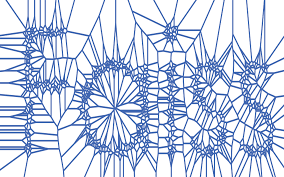
\includegraphics{images/faiss-vectorstore.png}%
    }
    \caption{FAISS vector store}
    \label{fig:faiss-vectorstore}
\end{figure}
\textbf{FAISS} là một thư viện được phát triển bởi Facebook AI Research, chuyên biệt cho việc tìm kiếm tương đồng (similarity search) và phân cụm (clustering). Điểm mạnh của FAISS nằm ở khả năng xử lý các vector embedding một cách hiệu quả, đồng thời cung cấp nhiều thuật toán và chỉ số (indexes) khác nhau để tối ưu hóa tốc độ và độ chính xác của quá trình tìm kiếm.

Trong hệ thống Chatbot của nhóm, \textbf{FAISS} đóng vai trò là nơi lưu trữ các vector embeddings của các chunks dữ liệu sản phẩm thảo dược.  Như đã đề cập ở phần \textbf{Xử lý dữ liệu}, sau khi dữ liệu sản phẩm được chia thành các chunks nhỏ bằng kỹ thuật Semantic Chunking, mỗi chunk sẽ được chuyển đổi thành một vector embedding. Các vector embedding này, mang trong mình thông tin ngữ nghĩa của từng chunk, sẽ được lưu trữ trong FAISS index.

Lý do nhóm chọn sử dụng một vector store chứ không phải một vector database là vì dữ liệu Chatbot phải xử lý là khá ít và tương đối đơn giản. Đồng thời trong bối cảnh đề tài này, nhóm chỉ có nhu cầu nhập và lưu trữ một lần thông tin và sau đó truy vấn nên việc sử dụng vector store sẽ nhanh và tiết kiệm tài nguyên hơn.
\subsection{Các phương pháp tìm kiếm}
Để truy xuất thông tin từ vector store FAISS một cách hiệu quả, nhóm đã triển khai và thử nghiệm ba phương pháp tìm kiếm chính:

\begin{itemize}
    \item \textbf{BM25} \cite{NguyenVanA2021BM25Viblo}, \cite{Robertson2009BM25Foundations} là một thuật toán xếp hạng tìm kiếm dựa trên mô hình xác suất, thường được sử dụng để đánh giá mức độ liên quan của các tài liệu đến một truy vấn tìm kiếm. Thay vì chỉ đơn thuần đếm số lần xuất hiện của từ khóa, BM25 xem xét tần suất từ (term frequency - TF) và tần suất nghịch đảo của tài liệu (inverse document frequency - IDF) để xác định tầm quan trọng của từ khóa trong một tài liệu và trong toàn bộ tập dữ liệu.
    
    Trong ngữ cảnh của Chatbot này, BM25 được sử dụng như một phương pháp tìm kiếm dựa trên từ khóa. Khi người dùng nhập một câu hỏi, hệ thống sẽ trích xuất các từ khóa quan trọng từ câu hỏi đó và sử dụng BM25 để tìm kiếm các chunks dữ liệu trong FAISS có chứa các từ khóa này. Các chunks dữ liệu được xếp hạng dựa trên điểm số BM25, và các chunks có điểm số cao nhất được coi là liên quan nhất đến truy vấn của người dùng.

    \item \textbf{Vector Similarity Search} sử dụng độ tương tự cosine (Cosine Similarity) để tìm kiếm các chunks dữ liệu liên quan đến truy vấn dựa trên ý nghĩa ngữ nghĩa của chúng, thay vì chỉ dựa trên sự trùng khớp từ khóa như BM25.
    
    Nhóm đã sử dụng hàm \texttt{similarity\_search} được triển khai sẵn trong thư viện của vector store \textbf{FAISS}.

    \item \textbf{Hybrid Search}\cite{NguyenHuuPhuoc2023SearchEngineVDB2} là phương pháp kết hợp cả Keyword Search (BM25) và Vector Search, sau đó áp dụng một mô hình \textbf{Reranker} để cải thiện độ chính xác của kết quả tìm kiếm. Quy trình Hybrid Search được thực hiện như sau:
    
    Đầu tiên, truy vấn của người dùng được sử dụng đồng thời cho cả hai phương pháp tìm kiếm: \textbf{BM25} và \textbf{Vector Search} để thu về hai tập kết quả ban đầu. Sau đó, hai tập kết quả này được hợp nhất để tạo thành một danh sách các tài liệu tiềm năng.
\end{itemize}

\subsection{Reranker}
Reranker~\ref{fig:reranker} là một thành phần quan trọng trong hệ thống Chatbot của nhóm, thành phần này được sử dụng để xếp hạng lại các thông tin, các tập tài liệu hoặc kết quả truy vấn đã được lọc sơ bộ. Mục tiêu chính của Reranker là cải thiện độ chính xác và mức độ liên quan của các tài liệu hoặc kết quả cuối cùng so với truy vấn đầu vào. Reranker đặc biệt hữu ích trong các hệ thống RAG để tinh chỉnh kết quả truy xuất ban đầu, vốn có thể còn nhiễu hoặc chưa hoàn toàn phù hợp với ý định của người dùng.

\begin{figure}[!ht]
    \centering
    \adjustbox{max width=1\linewidth, keepaspectratio}{%
        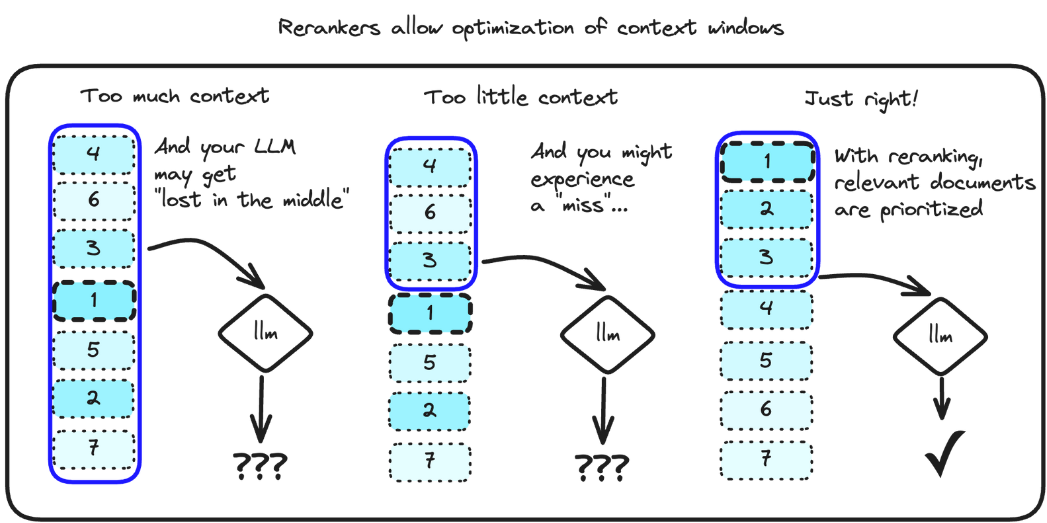
\includegraphics{images/reranker.png}%
    }
    \caption{Cách Reranker hoạt động}
    \label{fig:reranker}
\end{figure}

Trong đề tài này, sau khi truy xuất một tập hợp các chunks dữ liệu tiềm năng bằng các phương pháp Hybrid Search, nhóm sử dụng mô hình Reranker \texttt{BAAI/bge-reranker-v2-m3} để đánh giá lại mức độ liên quan của từng chunk dữ liệu so với câu truy vấn gốc. Mô hình \texttt{BAAI/bge-reranker-v2-m3}~\cite{FlagOpen2023} là một mô hình transformer được huấn luyện trước cho nhiệm vụ đo độ tương đồng ngữ nghĩa. Mô hình này nhận vào các cặp (truy vấn, chunk dữ liệu) và dự đoán điểm số liên quan. 

Bằng cách xếp hạng lại các chunk dữ liệu đã truy xuất dựa trên các điểm số này, nhóm hướng đến việc ưu tiên các chunk dữ liệu có ý nghĩa ngữ nghĩa sát với truy vấn của người dùng hơn, từ đó cải thiện chất lượng thông tin cung cấp cho mô hình ngôn ngữ lớn để tạo ra câu trả lời phù hợp cho khách hàng.

\section{\textbf{Đánh giá}}
\subsection{Phương pháp đánh giá}
Hiệu suất của hệ thông chatbot được đánh giá dựa trên các chỉ số định lượng, tập trung vào độ chính xác của kết quả trả về và hiệu quả xếp hạng. Dưới đây là một số độ đo mà nhóm sẽ sử dụng để đánh giá.

\textbf{Hit rate@k} đo tỷ lệ phần trăm của các truy vấn mà hệ thống có thể trả về ít nhất một kết quả đúng trong top k kết quả.

\textbf{MRR@k (Mean Reciprocal Rank)} là một độ đo dùng để đánh giá hiệu quả của một hệ thống truy xuất thông tin. Nó đo lường thứ hạng của kết quả đúng đầu tiên trong danh sách top k kết quả được trả về. Công thức được tính như sau:

\[
\text{MRR@k} = \frac{1}{N} \sum_{i=1}^{N} \frac{1}{\text{rank}_i}
\]

Trong đó:
\begin{itemize}
    \item N: Số lượng truy vấn
    \item $\text{rank}_i$: Thứ hạng của kết quả đúng đầu tiên trong top k cho truy vấn thứ $i$. Nếu không có kết quả đúng trong top k, giá trị MRR cho truy vấn đó bằng 0.
\end{itemize}

\textbf{NDCG (Normalized Discounted Cumulative Gain)} là một độ đo được sử dụng để đánh giá chất lượng của danh sách các kết quả được xếp hạng. NDCG không chỉ xét đến độ chính xác (relevance) của các kết quả, mà còn xem xét thứ tự mà các kết quả đúng xuất hiện. NDCG được tính dựa trên hai thành phần:

\begin{itemize}
    \item DCG (Discounted Cumulative Gain):
    \[
    \text{DCG@k} = \sum_{i=1}^{k} \frac{\text{rel}(i)}{\log_2(i+1)}
    \]
    Trong đó: 
    \begin{itemize}
        \item rel(i): độ liên quan (relevance) của kết quả tại vị trí thứ i trong top k kết quả.
        \item Với đề tài này thì rel(i) $\in \{0, 1\}$ thể hiện mức độ liên quan (có hoặc không).
    \end{itemize}

    \item IDCG(Ideal DCG): Đây là DCG của danh sách được sắp xếp hoàn hảo, tức là các kết quả đúng đều nằm ở đầu danh sách.
\end{itemize}

Từ hai thành phần trên, NDCG được tính bằng công thức:
\[
\text{NDCG@k} = \frac{\text{DCG@k}}{\text{IDCG@k}}
\]

Ngoài ra, nhóm sử dụng thêm một số độ đo phổ biến dưới đây:

\textbf{Recall@k} đo lường khả năng hệ thống trả về các kết quả đúng nằm trong top k so với toàn bộ kết quả đúng.

\textbf{Precision@k} đo lường tỷ lệ các kết quả đúng trong top k so với tổng số kết quả được trả về trong top k.

\textbf{F1-score@k} là trung bình điều hòa của \textbf{Recall@k} và \textbf{Precision@k}. Nó cân bằng giữa khả năng tìm đúng các kết quả và độ chính xác của top k.

\subsection{Bộ dữ liệu đánh giá}
Bộ dữ liệu đánh giá trong đề tài này được nhóm tự xây dựng và gán nhãn thủ công để đảm bảo chất lượng và độ chính xác. Bộ dữ liệu bao gồm 60 câu truy vấn, được thiết kế để bao quát nhiều lĩnh vực và loại sản phẩm khác nhau.

Đối với mỗi truy vấn, nhóm đã xác định thủ công một tập các tài liệu liên quan, được biểu diễn bằng chỉ số (index) của từng tài liệu. Các tài liệu liên quan được lựa chọn dựa trên mức độ phù hợp với nội dung truy vấn, đảm bảo phản ánh chính xác ngữ cảnh ngữ nghĩa và mục đích thông tin mà truy vấn hướng tới.

Hình~\ref{fig:evaluation_data} minh họa một vài câu truy vấn và tập các tài liệu liên quan đến nó được lấy từ bộ dữ liệu đánh giá.

\begin{figure}[!ht]
    \centering
    \adjustbox{max width=1\linewidth, keepaspectratio}{%
        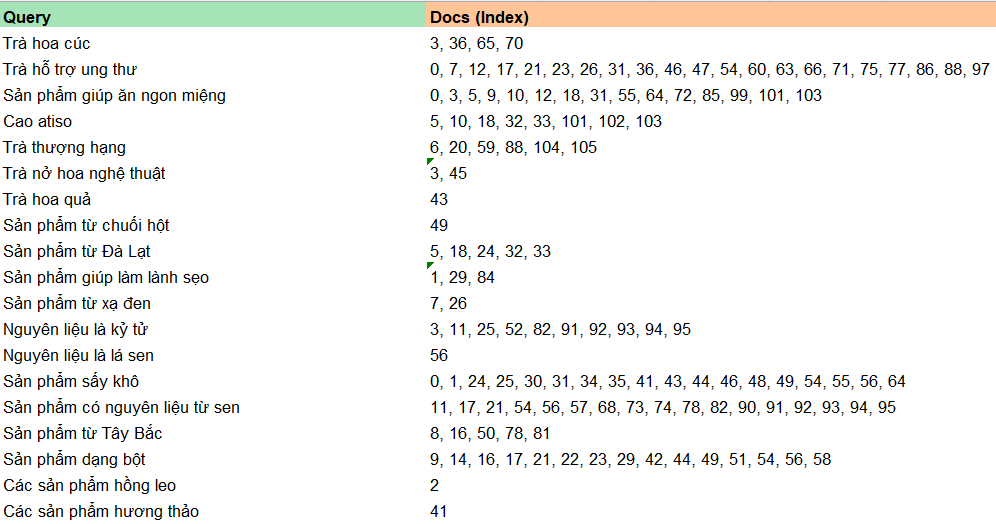
\includegraphics{images/evaluation_data.png}%
    }
    \caption{Hình ảnh một vài câu truy vấn đã được gán nhãn từ bộ dữ liệu đánh giá}
    \label{fig:evaluation_data}
\end{figure}

\subsection{Kết quả}
Trong phần này, chúng tôi trình bày và phân tích kết quả thực nghiệm dựa trên các embedding model, các phương pháp tìm kiếm và mô hình reranker được áp dụng. Các kết quả được đánh giá dựa trên bộ dữ liệu đánh giá mà nhóm đã đề cập ở phần trước với các chỉ số hiệu suất như Precision@k, Recall@k, F1-Score@k, MRR@k, Hit Rate@k và nDCG@k.

Bảng dưới đây thể hiện kết quả thực nghiệm của nhóm.

\begin{table}[!ht]
\centering
\resizebox{\textwidth}{!}{
\begin{tabular}{c c c c c c c c c c}
\toprule
\multicolumn{9}{c}{\textbf{text-embedding-3-small}} \\
\midrule
\textbf{Reranker} & \textbf{Embedding Model} & \textbf{Search Method} &  \textbf{Avg Prec\@10} & \textbf{Avg Rec\@10} & \textbf{Avg F1-Score\@10} & \textbf{Avg MRR\@10} & \textbf{Hit Rate\@10} & \textbf{Avg NDCG\@10} \\
\midrule
\multirow{6}{*}{\textbf{bge-reranker-v2-m3}} & \multirow{3}{*}{\textbf{halong-embedding}} & BM25 & 0.4391 & 0.6195 & 0.4466 & 0.8969 & 0.8969 & \textbf{0.9672} \\  
& & Similarity Search & 0.3038 & 0.4054 & 0.3022 & 0.8108 & 0.8689 & 0.6846 \\
& & Hybrid Search & \textbf{0.4474} & \textbf{0.6344} & \textbf{0.4537} & \textbf{0.9139} & \underline{0.9672} & 0.9424 \\
\cmidrule(lr){2-9}
& \multirow{3}{*}{\textbf{text-embedding-3-small}} & BM25 & 0.4391 & 0.6195 & 0.4466 & 0.8969 & \underline{0.9672} & 0.8778 \\
& & Similarity Search & 0.2803 & 0.3854 & 0.2803 & 0.7239 & 0.8361 & 0.6110 \\
& & Hybrid Search & 0.4397 & 0.6290 & 0.4463 & 0.9003 & \underline{0.9672} & 0.9203 \\
\midrule
\multirow{6}{*}{\textbf{PhoRanker}} & \multirow{3}{*}{\textbf{halong-embedding}} & BM25 & 0.4391 & 0.6195 & 0.4466 & 0.8267 & \underline{0.9672} & 0.8145 \\  
& & Similarity Search & 0.3038 & 0.4054 & 0.3022 & 0.7459 & 0.8689 & 0.6489 \\
& & Hybrid Search & 0.3933 & 0.5691 & 0.3975 & 0.8043 & \underline{0.9672} & 0.8082 \\
\cmidrule(lr){2-9}
& \multirow{3}{*}{\textbf{text-embedding-3-small}} & BM25 & 0.4391 & 0.6195 & 0.4466 & 0.8267 & \underline{0.9672} & 0.8415 \\
& & Similarity Search & 0.2803 & 0.3854 & 0.2803 & 0.6611 & 0.8361 & 0.5731 \\
& & Hybrid Search & 0.3988 & 0.5747 & 0.3993 & 0.8099 & \underline{0.9672} & 0.7958 \\
\bottomrule
\end{tabular}
}
    \label{table:result}
    \caption{Kết quả thực nghiệm}
\end{table}

Dựa vào bảng kết quả, nhóm có một số nhận xét như sau: 
\begin{itemize}
    \item Về mô hình embedding: \textbf{halong-embedding} hoạt động hiệu quả hơn trong hầu hết các trường hợp so với \textbf{text-embedding-3-small}, đặc biệt trong việc hỗ trợ với phương pháp tìm kiếm là BM25 và Hybrid Search. Điều này cho thấy mô hình embedding dành cho tiếng Việt hoạt động tốt hơn so với mô hình embedding đa ngôn ngữ (multilingual) trên bộ dữ liệu.
    \item Về các phương pháp tìm kiếm:
    \begin{itemize}
        \item BM25: Duy trì độ chính xác cao nhất trên nhiều chỉ số (Precision@10, F1-Score@10) khi sử dụng cả hai mô hình embedding. Điều này cho thấy phương pháp dựa trên từ khóa vẫn có hiệu quả trong ngữ cảnh tìm kiếm thông tin chính xác.
        \item Vector Search: Hiệu quả thấp hơn so với BM25 và Hybrid, đặc biệt là chỉ số nDCG@10. Điều này phản ánh rằng Vector Search cần sự hỗ trợ từ các phương pháp khác để cải thiện kết quả.
        \item Hybrid Search: Đạt hiệu suất tốt nhất trên hầu hết các chỉ số, đặc biệt là nDCG@10 và Hit Rate@10, chứng minh rằng việc kết hợp từ khóa và ngữ nghĩa mang lại kết quả toàn diện hơn.
    \end{itemize}
    \item Về mô hình reranker: \textbf{bge-reranker-v2-m3} cho kết quả tốt hơn \textbf{PhoRanker} trên hầu hết các chỉ số, đặc biệt là khi kết hợp với halong-embedding.
\end{itemize}

Với những phân tích trên, có thể thấy sự kết hợp của \textbf{halong-embedding}, phương pháp \textbf{Hybrid Search} và mô hình reranker \textbf{bge-reranker-v2-m3} là cho kết quả tốt nhất. Vì vậy, nhóm đã sử dụng sự kết hợp này để triển khai ứng dụng.

\section{\textbf{Tổng kết}}
Qua quá trình nghiên cứu và triển khai, nhóm đã xây dựng thành công một hệ thống chatbot ứng dụng công nghệ Retrieval-Augmented Generation (RAG) để tư vấn khách hàng về các sản phẩm thảo dược. Hệ thống được thiết kế tối ưu, kết hợp các kỹ thuật tiên tiến như Semantic Chunking, Vector Store FAISS, và Hybrid Search, đồng thời áp dụng mô hình reranker hiện đại để đảm bảo tính chính xác và liên quan của kết quả truy vấn.

Kết quả đánh giá cho thấy hệ thống hoạt động hiệu quả với các chỉ số cao về độ chính xác, độ liên quan và hiệu suất xếp hạng. Sự kết hợp giữa \textbf{halong-embedding}, Hybrid Search, và \textbf{bge-reranker-v2-m3} đã mang lại kết quả tối ưu, chứng minh tính khả thi và giá trị thực tiễn của giải pháp.

Hệ thống không chỉ giúp nâng cao trải nghiệm khách hàng nhờ khả năng tư vấn nhanh chóng và chính xác, mà còn giảm tải công việc cho nhân viên, góp phần thúc đẩy sự phát triển của AI trong lĩnh vực kinh doanh thảo dược. Trong tương lai, nhóm hướng đến việc mở rộng quy mô dữ liệu và tích hợp thêm các tính năng mới để nâng cao khả năng phục vụ, đồng thời tối ưu hóa hiệu quả vận hành của hệ thống chatbot.

\begin{figure}[!ht]
    \centering
    \adjustbox{max width=1\linewidth, keepaspectratio}{%
        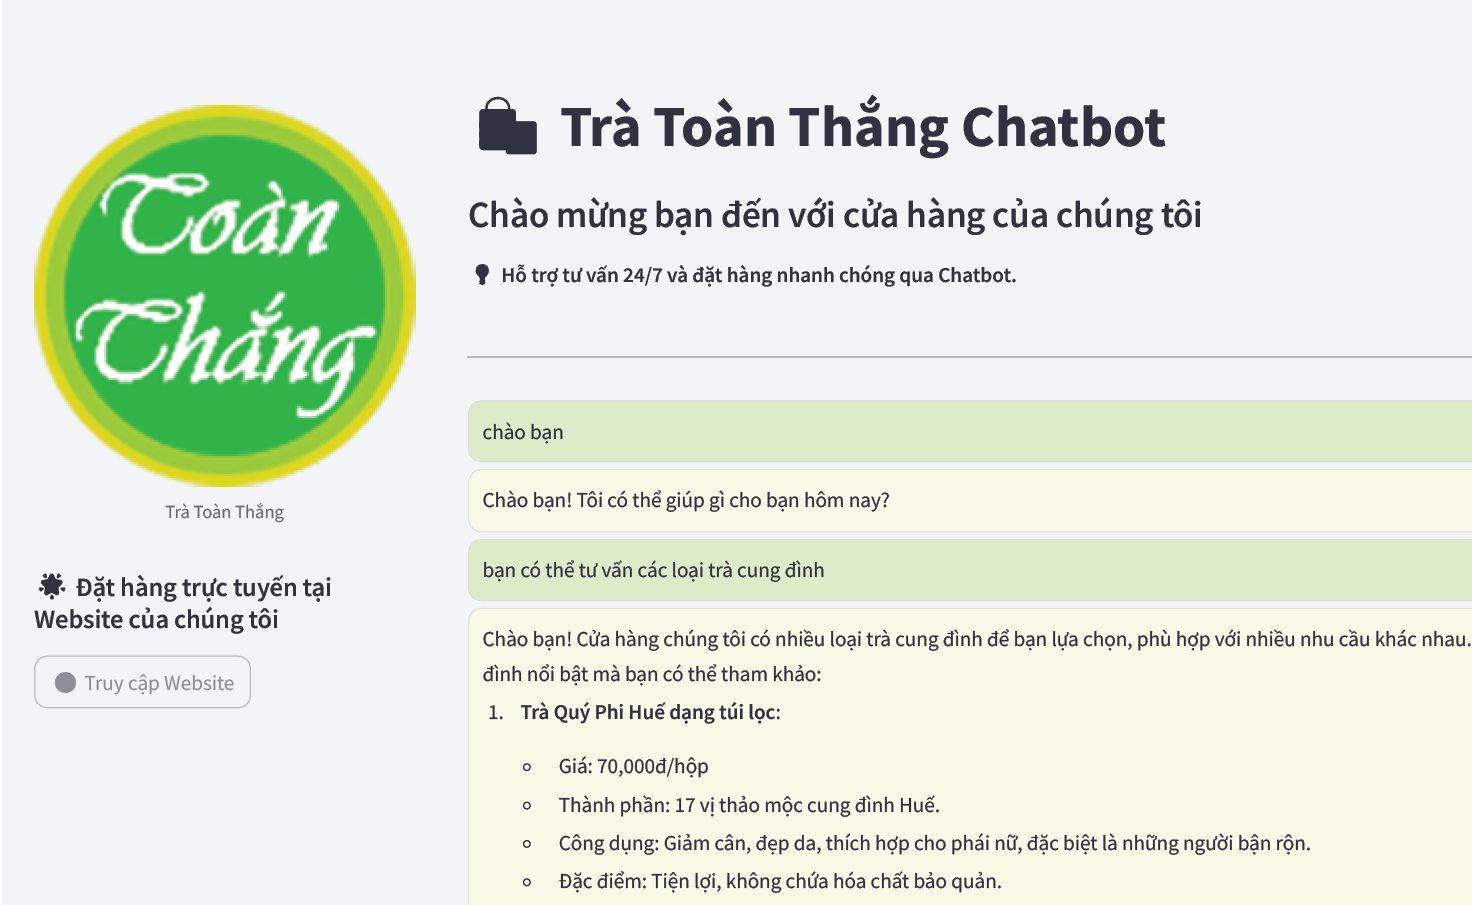
\includegraphics{images/interface.png}%
    }
    \caption{Giao diện của hệ thống chatbot được nhóm triển khai}
    \label{fig:interface}
\end{figure}
\newpage
\nocite{rotonx-ai-devs-02_cuongtm-vietnamese-rag-chatbot}
\nocite{protonx-ai-devs-02_quynhtl-owndata-rag-bot}
\printbibliography
\end{document}

